\chapter{Implementation}

The following chapter describes how the protoype has been implemented and the materials needed to build the prototype. 

\section{Theory}

This section explains the theory behind the effects that has been used in the implementation. 
%Write about pitchshifting and stuff, not code


\section{Hardware and Software}

This sections describes the hardware that has been used. It also explains the software part of the prototype. 

\subsection{Hardware}

The prototype consists of an Arduino Mega 2560\citep{Arduino}, with a connection to a circuit board with an inertial measurement unit(IMU). 
The IMU uses the MPU 9150 sensor with 9 degrees of freedom\citep{MPU}. It has a tri-axis gyroscope, magnetometer, and accelorometer.

\subsection{Schematic} 

The following figure \ref{schematic} shows the connection from the Arduino to the circuit board with the IMU. The black switch at the top of the circuit board
represents the three connections, which is put on the thumb, index and middle finger. These are velcro based, with copper tape on them, to create the connection when pressed together. 

\begin{minipage}{\linewidth}% to keep image and caption on one page
\makebox[\linewidth]{%        to center the image
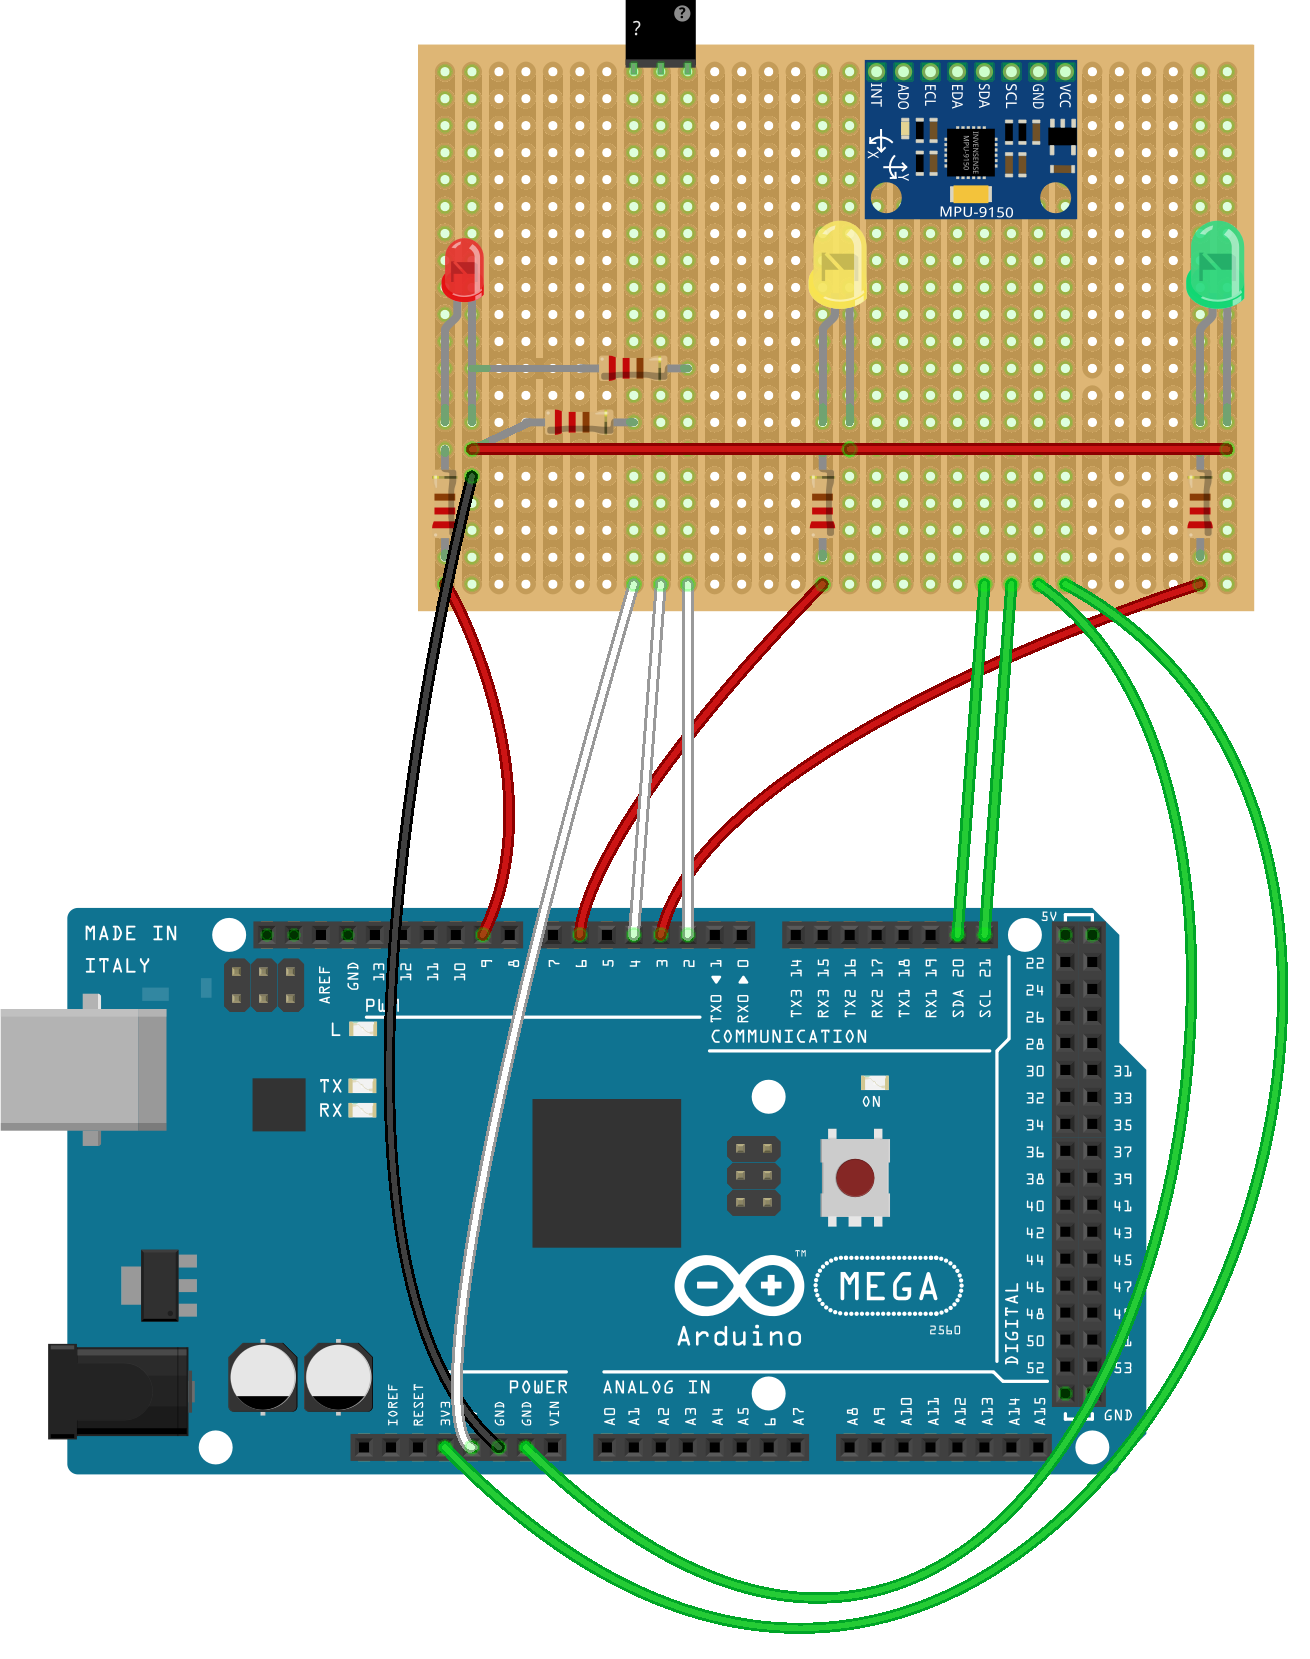
\includegraphics[keepaspectratio=true,scale=1]{Imu_Glove_Schematic}}
\captionof{figure}{Prototype Schematic}\label{schematic}
\end{minipage}\\

The circuit board consists of three LEDs, a yellow, green and red. They light up at different points, which is explained in the next section of this chapter.
The LEDs are connected to resistors of 220 Ohm which is wired to the arduino as seen in the schematic. The green LED is connected to pin 3. 
The yellow LED is connected to pin 6 and the red is connected to pin 9. This is essential to make it work in the Arduino code, which will be described later. 
The black wire connects all the LEDs and runs from them, to the ground on the Arduino. The blue circuit board represents the IMU. The necessary connections are: SDA, SCL, GND and VCC. 
The SDA connection is connected to pin 20 and the SCL is connected to pin 21. GND is connected to ground on the Arduino and the VCC connection powers the sensor and is therefore
connected to 3.3V on the Arduino. The white wires are also connected to the Arduino. The first wire from the left, which goes to the thumb, is connected to the 5V on the Arduino. 
The white wire beside it, is connected to the index finger, and pin four on the Arduino. The last white wire is connected to the middle finger and pin two on the Arduino.
The wire which is connected to the thumb creates a circuit to the LEDs whenever the connection is created between either the thumb and index finger or thumb and middle finger. \\


The LEDs has to be connected to a pull-down resistor\citep{Pulldown_res}, which makes sure, that the Arduino does not 'float' between two different values. A pull-down resistor ensures, that the value is zero, when no active device is connected.
The following figure \ref{Pull_down} shows what a circuit with a pull-down resistor might look like. \\


\begin{minipage}{\linewidth}% to keep image and caption on one page
\makebox[\linewidth]{%        to center the image
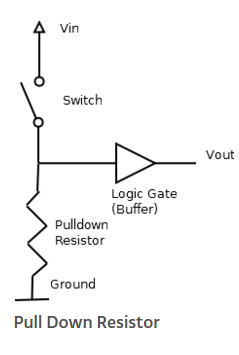
\includegraphics[keepaspectratio=true,scale=0.7]{Pull_down_resistor}}
\captionof{figure}{Schematic of Pull-down resistor\citep{Pull_down_res}}\label{pull_down}
\end{minipage}\\



The following figure shows the prototype. As one can see, the velcro for the fingers has copper tape on it, which has been glued onto the velcro. The velcro enables the user to wear the glove, and use it properly.  
This means that whenever the copper tape gets connected with the copper tape on the thumb, it creates the connection as mentioned earlier. 
The prototype has cloth sewed onto it, which makes it possible to wrap it around the wrist. 
%Picture of prototype maybe?


\subsection{Software}

The following section describes the software part of the implementation. 

\subsubsection{Arduino}
The Arduino language is based on C/C++, and whenever a sketch is compiled, it is sent to a C/C++ compiler \citep{Arduino_FAQ}.\\

Figure \ref{while_loop} shows a part of the code in Arduino. The specific code in the figure, is a while-loop, which reads the data from the IMU sensor and displays it.
This information is translated into values which is used to determine the pitch or harmoniser. \\

\begin{minipage}{\linewidth}% to keep image and caption on one page
\makebox[\linewidth]{%        to center the image
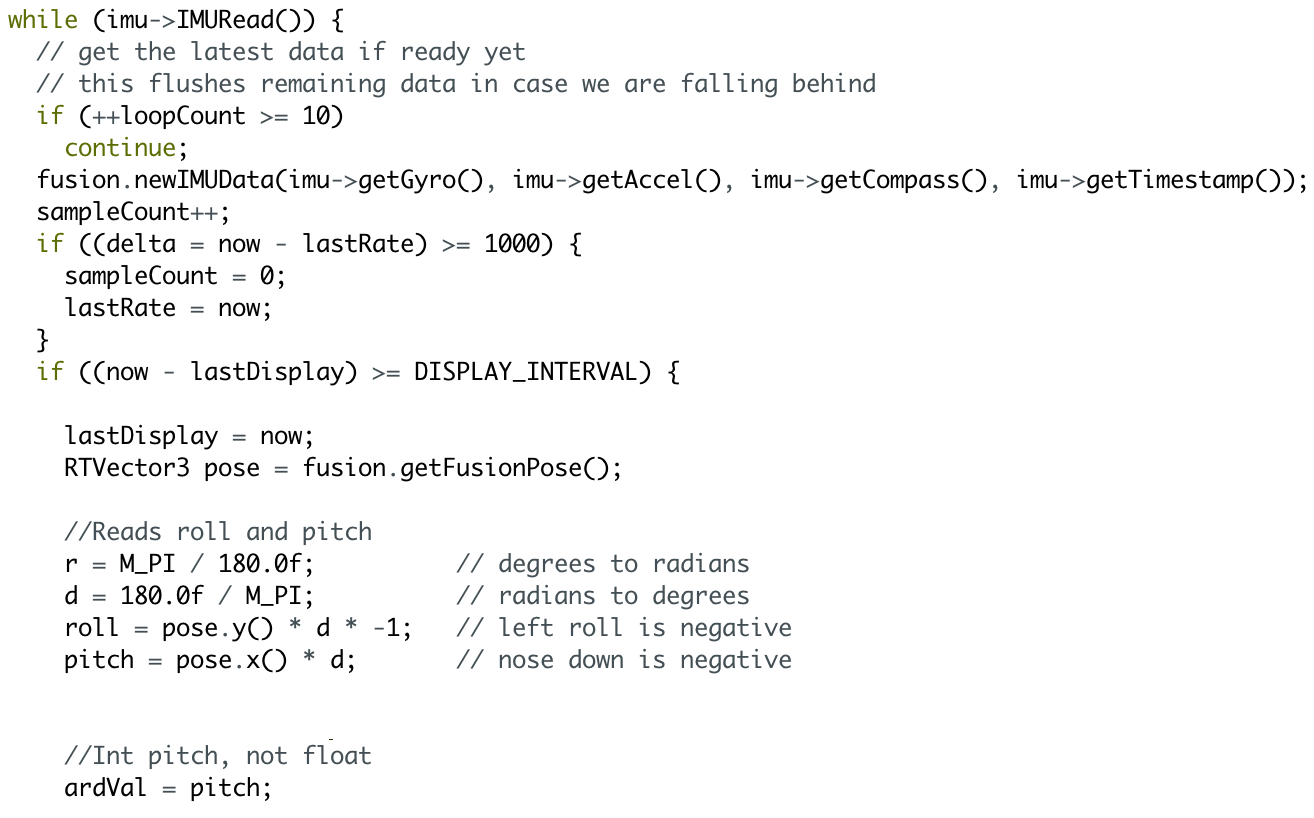
\includegraphics[keepaspectratio=true,scale=0.5]{Arduino_while_loop}}
\captionof{figure}{While loop}\label{while_loop}
\end{minipage}\\

The first part of the code in figure \ref{index_finger} reads the state of the copper plates. The following if-statement is executed whenever the index finger is connected. 
If one turns the hand to the left, the code sends the information to PureData, and if the hand is turned to the right, it sends that information. 
The direction of the hand determines the pitch within a value of 0-255. The motion is a rolling motion, which resembles the motion of turning a knob. 
The code used for the middle finger is almost identical. It does however use different pins. \\ 


\begin{minipage}{\linewidth}% to keep image and caption on one page
\makebox[\linewidth]{%        to center the image
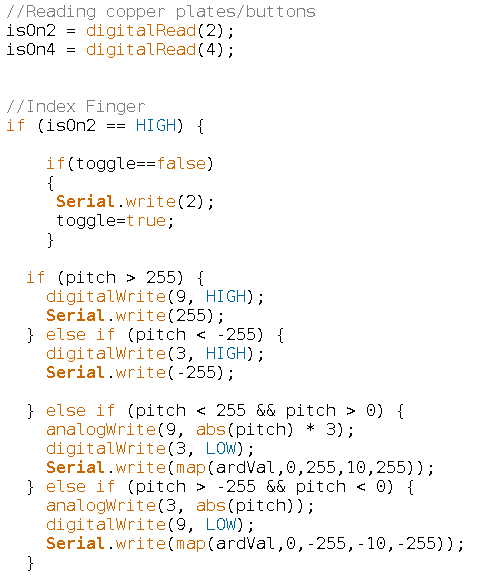
\includegraphics[keepaspectratio=true,scale=0.5]{Ardunio_Index_Finger}}
\captionof{figure}{Defining what happens when the index finger is connected}\label{index_finger}
\end{minipage}\\

The following figure \ref{Arduino_else} shows the last part of the code. This is an else statement that makes sure that the button is off whenever the copper plate is released. 

\begin{minipage}{\linewidth}% to keep image and caption on one page
\makebox[\linewidth]{%        to center the image
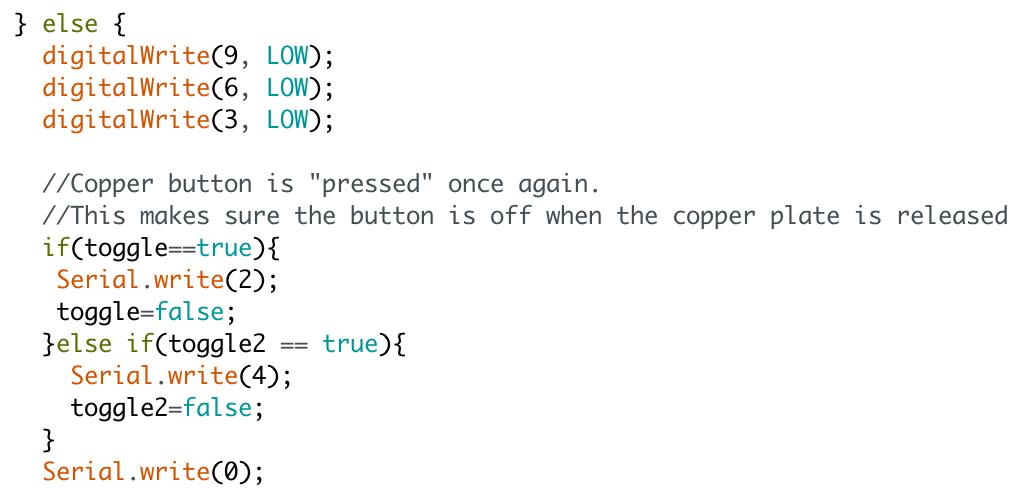
\includegraphics[keepaspectratio=true,scale=0.5]{Ardunio_else}}
\captionof{figure}{Else statement which makes sure the button is off when released}\label{Arduino_else}
\end{minipage}\\


\subsubsection{PureData}

The audio processing has been done in PureData(PD)\citep{PD_Info}, which is an open source programming language. It is used to generate and process sound, in a graphical way. 
The program uses patches where one can create objects which makes it possible to create different audio effects. The following subsection describes how PD has been used in this project,
and explains the patches made for this project. \\

The follwing figure \ref{PitchShifting_PD} shows the pitch shifting patch made in PD. 


\begin{minipage}{\linewidth}% to keep image and caption on one page
\makebox[\linewidth]{%        to center the image
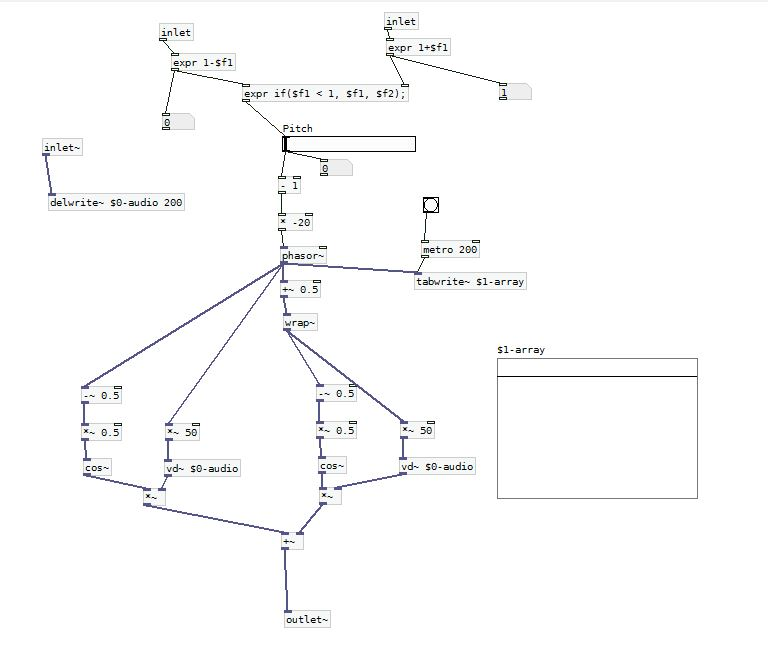
\includegraphics[keepaspectratio=true,scale=0.5]{PitchShifting_PD}}
\captionof{figure}{Pitchshifting in PureData}\label{PitchShifting_PD}
\end{minipage}\\

The patch uses the input, which might be comming from a microphone input. The slider called pitch shows how much the voice is actually being pitched. 